%!TEX root = paper.tex

\section{Introduction} % (fold)
\label{sec:introduction}
Automatic loop invariant generation is a fundamental program analysis. A loop invariant can be useful for software verification, test-case generation, compiler optimization, program understanding, etc.
Many approaches have bee proposed for invariant generation, e.g., based on abstraction interpretation~\cite{cite}, based on counterexample guided abstraction refinement~\cite{cite}, using interpolation-based approaches~\cite{cite}, and based on constraint-based inference~\cite{cite}. In~\cite{sharma2012interpolants,DBLP:conf/sas/0001GHAN13,sharma2014invariant}, the authors propose to automatically generate loop invariants based on random searching~\cite{sharma2014invariant} as well as machine learning~\cite{sharma2012interpolants}. The idea is to obtain sample program states in the loop and generalize the program states in certain way (e.g., through classification~\cite{sharma2012interpolants,DBLP:conf/sas/0001GHAN13}) to guess a candidate loop invariant (e.g., a classifier). The candidate loop invariant is then checked using program verification techniques) to see whether they are inductive and strong enough to prove the program property. If the checking fails, often with a counterexample, the guess-and-check iteration is repeated until a correct invariant is generated. One problem of the above approach is that its effectiveness is often limited by the sample program states obtained. In order to guess the correct invariant through classification, often program states right by the actual classifier must be sampled so that classification techniques would identify it. Otherwise, through random sampling, it is often unlikely that those specific program states would be sampled. As a result, many iterations of guess-and-check would be necessary so that the candidate candidate converges to the actual one.

In this work, we propose a framework for loop invariant generation through iterations of active learning and checking. Through active learning, we aim to improve the quality of the generated candidate loop invariants every iteration prior to employing heavy techniques like program verification. As a result, we can reduce the number of guess-and-check iterations significantly. Furthermore, by supporting an extensible framework, we can easily integrate different classification techniques (e.g., SVM with kernel methods~\cite{}) as well as active learning techniques. %We have developed a prototype implementation of our method and applied to benchmark programs including those from the software verification competition. The results show that our method often reduces the number of guess-and-check iterations as well as is able to learning more loop invariants than existing approaches.
In the following, we define our problem and briefly illustrate how our approach works.

\paragraph{Problem Definition} We assume that we are given a Hoare triple in the following form:
%\[
%    P = \{ \mathit{Pre} \} \mathit{while}(\mathit{Cond}) \{ \mathit{Body} \} \{ \mathit{Post} \}
%\]
\begin{align*}
&\{\mathit{Pre}\} & & /\star\text{\emph{Assumption}}\star/ \\
&\mathit{while} (\mathit{Cond}) \{ \mathit{Body} \} && /\star\text{\emph{Loop Body}}\star/\\
&\{\mathit{Post}\} & & /\star\text{\emph{Assertion}}\star/
\end{align*}
Assume that $V = \{x_1, x_2, \cdots, c_n\}$ is a finite set of relevant variables. $\mathit{Pre}$, $\mathit{Cond}$ and $\mathit{Post}$ are predicates constituted by variables in $V$. $\mathit{Body}$ is an imperative program which potentially updates the valuation of $V$.
%In practice, the pre-condition $\mathit{Pre}$ is often described by
%the specification documents and checking conditions of the program inputs,
%and the post-condition $\mathit{Post}$ is usually specified
%by assertions and exceptions leading to an error state in the program.
Let $s = \{ x_1 \mapsto v_1, \ldots, x_n \mapsto v_n \}$ be a valuation of $V$. Let $\phi$ be a predicate constituted by variables in $V$. We write $s \models \phi$ to denote that $\phi$ valuates to true given the program state $s$. We write $s \not \models \phi$ otherwise. For simplicity, we assume that $\mathit{Body}$ is a deterministic function on valuations of variables $V$. Thus, we write $\mathit{Body}(s)$ to denote the valuation of $V$ after executing $\mathit{Body}$ with initial variable valuation $s$.
%the evaluation function of the program variables $x_1, \ldots, x_n$
%and $\mathit{Body}(s)$ stand for their new evaluation after the execution of $\mathit{Body}$,
%the above program means that (1) $\mathit{Pre}$ is the assumption to the initial value of $s$;
%(2) if the $\mathit{Cond}$ is satisfied by $s$ at an iteration,
%$\mathit{Body}$ will be executed and $s$ will be updated to $\mathit{body}(s)$;
%(3) if the $\mathit{Cond}$ is unsatisfied by $s$ at an iteration,
%the while-loop ends and $s$ should satisfy $\mathit{Post}$.
Our problem is to either prove the Hoare triple or disprove it. In order to prove the Hoare triple, we would like to find a loop invariant $\mathit{Inv}$ that satisfies the following three conditions.
\begin{align}
    &s \models \mathit{Pre}
        &&\Longrightarrow & s &\models \mathit{Inv} \label{inv:pre} \\
    &s \models \mathit{Inv} \wedge \mathit{Cond}
        &&\Longrightarrow & \mathit{Body}(s) &\models \mathit{Inv} \label{inv:loop} \\
    &s \models \mathit{Inv} \wedge \neg\mathit{Cond}
        &&\Longrightarrow & s &\models \mathit{Post} \label{inv:post}
\end{align}
For simplicity, we assume that the given program is always terminating. We refer the readers to~\cite{} for the extensive research on proving loop termination.
Alternatively, we would like to find a valuation $s$ such that $s \models \mathit{Pre}$ and executing the loop until it terminates results in a state $s'$ such that $s' \models \mathit{Post}$ is not true. The goal of this work is to develop a way of automatically identifying an $\mathit{Inv}$ to prove the Hoare triple or finding a valuation $s$ to disprove it.

\paragraph{Contributions.} In solving the above problem, we make the following contributions in this work.
\begin{itemize}
    \item
    We are the first to propose an active learning and refinement framework
    for automatic invariant inference based on machine learning.
    Since the samples are chosen for clear purpose
    to refine the invariant candidate in the \emph{data collection} stage,
    the invariant converges efficiently.
    Furthermore, because the counter-examples generated in the \emph{invariant verification} stage
    give very accurate information to amend the invariant candidate,
    they become a useful supplementary to overcome the weakness of machine learning
    and fine-tune the invariant candidate.
    \item
    Our framework is highly adaptable to different invariant inference scenarios
    because the classification methods have a wide range of choices.
    In this work, we show that linear, polynomial as well as
    their conjunctive classification methods work effectively in our framework.
    More importantly, our framework can be easily and intuitively extended with other alternative methods.
    \item
    Our framework can be practically used to verify real programs with ease,
    as the samples are generated at runtime
    and our framework is language/platform independent based on other tools
    (e.g., GSL (GNU Scientific Library)~\cite{gough2009gnu} for selective sampling,
    LibSVM~\cite{chang2011libsvm} for SVM classification,
    Z3~\cite{de2008z3} for invariant verification
    and KLEE~\cite{cadar2008klee} for concolic testing~\cite{sen2007concolic}).
    \item
    We implement our framework as a tool called \textsc{Zilu}
    and compare it with other available state-of-the-art invariant inference tools,
    i.e., CPAChecker~\cite{beyer2011cpachecker}, Interproc.
    Our experiment results show that
    we are the only tool that can work with polynomial invariant inference.
    Notice that the polynomial invariant inference works in our framework
    naturally with very light additional programming.
    % Based on the design of different approaches,
    % we also claim that our framework have better extensibility comparing with their method.
\end{itemize}


\paragraph{Organization} The remainders of the paper are organized as follows. Section~\ref{sec:overview} presents an overview of our approach using an illustrative example. Section~\ref{sec:sampling} to~\ref{sec:verification} present the details of our approach step-by-step. Section~\ref{sec:evaluations} discusses our prototype implementation and evaluates its effectiveness using a set of benchmark programs including those from the software verification competition~\cite{}. Lastly, Section~\ref{sec:related} reviews related and concludes.

\section{Overview} \label{sec:overview}
In the following, we use a simple example to illustrate how our approach works. The Hoare triple is shown in Figure~\ref{fig:running:example:program} (where an $assume$ statement captures the pre-condition and an $assert$ statement captures the post-condition). The set of variables $V$ contains two integer type variables $X$ and $Y$. For simplicity, in this work, we interpret integers in the programs as mathematical integers (which do not overflow). The pre-condition $Pre$ is $x < y$, which is the same as the loop condition $Cond$.
During each loop iteration, $x$ is increased by $7$ if it is negative; otherwise it is increased by $10$. $y$ is decreased by $10$ if it is negative; otherwise it is increased by $3$. The postcondition is that $y \le x \le y + 16$.
The Hoare triple can be proven using a loop invariant like $Inv = x \le y + 16$. In the following, we show how our framework works to learn a similar loop invariant which would allow us to prove the Hoare triple.

In our framework, loop invariant generation is an active learning and refinement process based on iterations of data collection, active learning and invariant verification. The overall workflow is shown in the Figure~\ref{fig:overview}. There are three main stages: data collection, active learning and invariant verification.

We start with the data collection stage. Given the Hoare triple, we first randomly sample variable valuations based on $\mathit{Pre}$, e.g., using a constraint solver to obtain variable valuations which satisfy or dissatisfy $\mathit{Pre}$. For each sampled valuation $s_0$, we execute the given program with initial variable valuation $s_0$ and record the variable evaluations after each iteration of the loop as a trace $\langle s_0, s_1, \ldots, s_n \rangle$ where $s_n \not \models \mathit{Post}$. Let $T$ denote the set of traces. We write $s \Rightarrow_T s'$ to denote that there exists a trace $\langle s_0, s_1, \cdots, s, \cdots, s', \cdots, s_n \rangle \in T$.
All variable valuations in the traces are then divided into four categories.
\begin{itemize}
    \item Set $Counterexample = \{s | s \models Pre \land s \Rightarrow_T s' \land s' \not \models Post\}$ contains the set of valuations which satisfy the precondition and violate the postcondition afterwards. We remark that anytime a program state in $Counterexample$ is identified, a counterexample is found and the Hoare triple is disproved.
    \item Set $Positive = \{s | s \models Pre \land s \Rightarrow s' \land s' \models Post\}$ contains the set of valuations which satisfy the precondition and the postcondition afterwards. We remark for every valuation $s \in Positive$ such that $s \models Cond$, $s \models Inv$.
    \item Set $Negative = \{s | s \not \models Pre \land s \Rightarrow s' \land s' \not \in Post\}$ contains the set of valuations which do not satisfy the precondition or the postcondition afterwards. We remark for every valuation $s \in Negative$, $s \not \models Inv$.
    \item Set $NP = \{s | s \not \models Pre \land s \Rightarrow s' \land s' \models Post\}$ contains the set of valuations which do not satisfy the precondition but satisfy the postcondition afterwards. We remark that a valuation $s \in NP$ may or may not satisfy $Inv$.
\end{itemize}
% Otherwise, because $Inv$ must satisfy (1),(2) and (3), we know that $P_T \subseteq Inv$ and $N_T \cap Inv = \emptyset$. The program states in $NP_T$ may or not may be in $Inv$. If we know that a program state $s \in NP_T$ is in $Inv$, $Body^*(s) \subseteq Inv$.
%
%Each trace is then associated with a pair of boolean labels $(SatPre, SatPost)$
%
%    All of the evaluations in the above trace (referred by its initial evaluation $s_0$)
%    are labelled based on a pair of boolean values
%    $(s_0 \models \mathit{Pre}, s_n \models \mathit{Post})$\footnote{
%        $(\mathit{true}, \mathit{true}) \rightarrow +$,
%        $(\mathit{false}, \mathit{false}) \rightarrow -$
%        and $(\mathit{false}, \mathit{true}) \rightarrow ?$}.
Assume that the following two valuations are generation in our running example: $\{x \mapsto 1, y \mapsto 2\}$ and $\{x \mapsto 100, y \mapsto 0\}$. Two traces are generated accordingly: $\langle \{x \mapsto 1, y \mapsto 2\}, \{x \mapsto 11, y \mapsto 5\} \rangle$ and $\langle \{x \mapsto 100, y \mapsto 0\} \rangle$. As a result, the set $Positive$ contains $\{x \mapsto 1, y \mapsto 2\}$; $Negative$ is empty; and $NP$ contains $\{x \mapsto 100, y \mapsto 0\}$. 

\begin{figure}[t]
\begin{subfigure}{0.5\textwidth}
    \raggedright
    \vspace{0.5cm}
{\scriptsize\begin{verbatim}
void P(int x, int y) {
    assume(x < y);
    while (x < y) {
        if (x < 0) x = x + 7;
        else x = x + 10;

        if (y < 0) y = y - 10;
        else y = y + 3;
    }
    assert(x >= y
        && x <= y + 16);
}
\end{verbatim}}
    \vspace{0.5cm}
    \caption{Loop Program}
    \label{fig:running:example:program}
\end{subfigure}%
\begin{subfigure}{.5\textwidth}
      \centering
      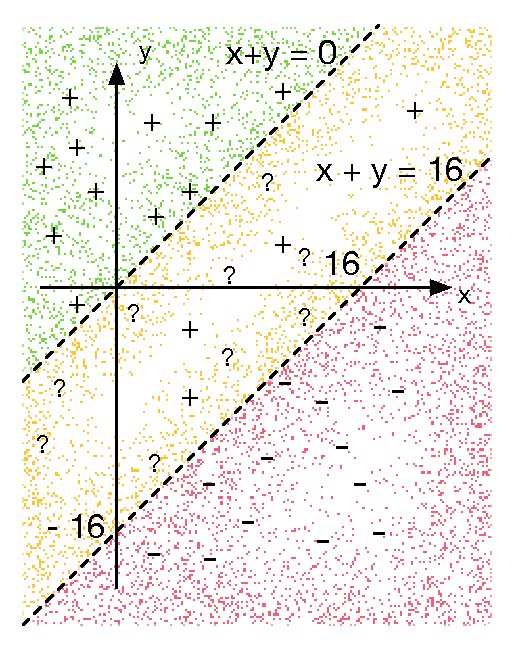
\includegraphics[scale=0.42]{figures/running-sampling.pdf}
      \caption{Sampling}
      \label{fig:running:example:sampling}
\end{subfigure}
\caption{A running example}
\label{fig:running:example}
\end{figure}

\begin{figure}[t]
    \centering
    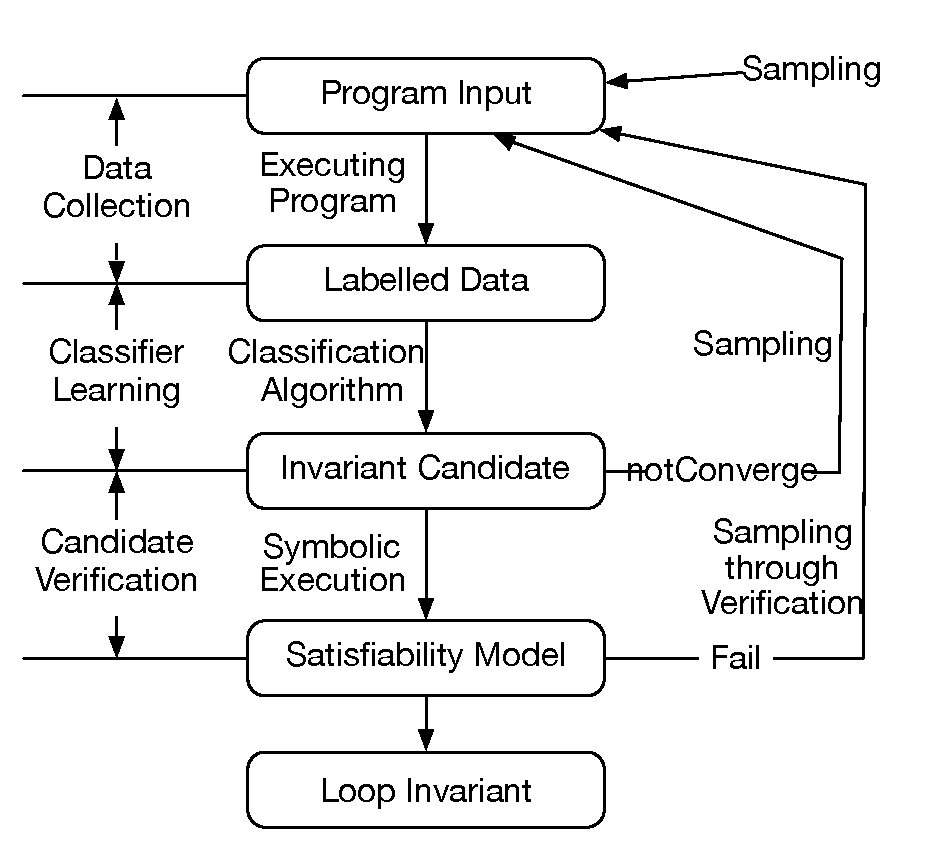
\includegraphics[scale=0.45]{figures/overview.pdf}
    \caption{Loop Invariant Inference Framework Overview}
    \label{fig:overview}
\end{figure}

In the \textbf{active learning} stage, with the three sets of valuations $Positive$, $Negative$ and $NP$, we apply active learning techniques to learn a classifier to capture the positive ones from the negative ones
    using machine learning algorithms, e.g., SVM derivatives.
    When the recently learnt classifier converges to the previously learnt ones,
    we treat it as an invariant candidate and move to the next stage.
    Otherwise, we apply selective sampling on the recently learnt classifier
    to add more samples to $S_{\mathit{in}}$.
    When a sample cannot be classified using a certain classification model,
    we try other alternative models in a sequential order.
    \LL{We prove the termination of the \emph{active learning} stage if such an invariant exists.}

Figure~\ref{fig:running:example:sampling} shows where the set of valuations in $Positive$, $Negative$ and $NP$ geographically in a plane for our running example, where valuations in $Positive$ are labeled with $+$ and color green; and valuation in $Negative$ are labeled with $-$ and color red; and valuations in $NP$ are labeled with ? and color yellow. Note that it can be observed the line separating the red region and the rest is correlated to the loop invariant that we are searching for.


    In the \textbf{Invariant Verification} stage (see Section~\ref{sec:verification}),
    we check the correctness of the invariant candidate.
    First, we check condition (\ref{inv:pre}) and condition (\ref{inv:post}) with the candidate.
    Then, we verify the condition (\ref{inv:loop})
    based on all of the program execution traces of $\mathit{Body}$ using symbolic execution~\cite{}.
    The above conditions are checked by SMT~\cite{barrett2009satisfiability} solvers in this work.
    If all of the above conditions are satisfied,
    we claim the correctness of $P$ with its loop invariant.
    Otherwise, we add the counter-example from SMT Solving to $S_{\mathit{in}}$
    and restart from the \emph{data collection} stage.

%The overall algorithm is shown in Algorithm~\ref{alg:overall}.
%\section {Overall Algorithm}
%\label{sec:overall}
% \LL{Do not put the algorithm here. It contains lots of notations undefined.}
% The overall algorithm is presented in Figure~\ref{alg:overall}.
% \begin{algorithm}[!h]
% \SetAlgoVlined
% \Indm
% \KwIn{$Pre$, $Cond$, $Body$, $Post$}
% \KwOut{an invariant which completes the proof or a counter-example}
% \Indp
% let $S$ be \textsc{Null}\;
% \While{true} {
%     add Samples into $S$\;
%     test the program for each sample in $S$\;
%     \If {a state $s$ in $\mathcal{S}^x$ is identified} {
%         \Return $s$ as a counterexample;
%     }
%     let $\mathcal{S}^+$, $\mathcal{S}^-$ and $\mathcal{S}^\rightarrow$ be respective sets accordingly\;
%     let $\mathcal{C}$ = activeLearning($\mathcal{S}^+$, $\mathcal{S}^-$, $\mathcal{S}^\rightarrow$)\;
%     Extract path constraints $\textsc{Pc}$ based on (1)(2)(3)\;
%     \For {each $pc$ in $\textsc{Pc}$} {
%         \If { $pc$ is not satisfied} {
%             add the counter-example into $S$\;
%             continue\;
%         }
%     }
%     \Return $\mathcal{C}$ as the proof;
% }
% \caption{Algorithm $overall$}
% \label{alg:overall}
% \end{algorithm}
%
% \begin{theorem}
% Algorithm $overall$ always eventually terminates and it is correct. \hfill \qed
% \end{theorem}


